\documentclass[10pt, a4paper, english]{article}
\usepackage{babel}
\usepackage{amsfonts} 
\usepackage{amsmath}
\usepackage{tikz}
\usepackage{graphicx}
\usepackage{hyperref}
\usepackage{titlesec}
\usepackage{changepage}
\usepackage{setspace}
\usepackage[a4paper, margin=1.15cm]{geometry}
\usepackage{multicol}
\usepackage[x11names]{xcolor}
\usepackage{fontawesome5}
\usepackage{paracol}
\usepackage{lipsum}
\usepackage{calc}
\usepackage[shortlabels]{enumitem}

%\usepackage{cmbright}
\usepackage[OT1]{fontenc}
\renewcommand*\familydefault{\sfdefault}

\renewcommand{\baselinestretch}{1.3} 


\hypersetup{
    colorlinks=true,
    linkcolor=black,
    filecolor=magenta,      
    urlcolor= DodgerBlue4,%cyan,
    pdftitle={CV Oscar Karlsson},
    pdfauthor ={Oscar Karlsson},
    pdfpagemode=FullScreen,
    }
\urlstyle{same}
\titleformat*{\section}{\normalsize\bfseries}

\def\makeemail{~\href{mailto:osc16kar@gmail.com}{osc16kar@gmail.com} }
\def\makegit{~\href{https://github.com/Squid-oid}{github.com/Squid-oid} }
\newcommand{\smallgit}[1]{~\href{#1}{\faGithub} }
\def\makeLinkedin{~\href{https://www.linkedin.com/in/oscar-karlsson-469044164}{in/oscar-karlsson-469044164} }

\def\MastersTitle{Master's Thesis -- Better hedging of CVA with reinforcement learning}%~\href{http://lup.lub.lu.se/student-papers/record/9197473}{ \scriptsize \faLink}

\newcommand{\mysection}[1]{\color{black}\textbf{\LARGE{#1}}\\
				        \rule[1em]{\widthof{\textbf{\LARGE{#1}}}}{1.333pt} \color{darkgray!80!black}\\ \vspace{-1em}}
\newcommand{\WExperience}[4]{\normalsize \noindent \textbf{#1}\hfill #3 \newline \textit{\footnotesize #2} \hfill \textit{\footnotesize #4} \vspace{-0.35em}}
\newcommand{\PExperience}[3]{\normalsize \noindent \textbf{#1} $\vert$ \textit{\footnotesize#3} \hfil \\ #2 \vspace{-0.25em}}
\author{Karlsson, Oscar}


\begin{document}
%no page numbers, column setup
\pagenumbering{gobble}
\columnratio{0.3}
\colseprulecolor{LavenderBlush3}
\setlength{\columnsep}{1.5em}
\setlength{\columnseprule}{4.5pt}

%%%%%%%%%%%%%%%%%%%%%
% Start work in the left column, right align text
%%%%%%%%%%%%%%%%%%%%%
\begin{paracol}{2}
%% Set up profile picture with 
\raggedright
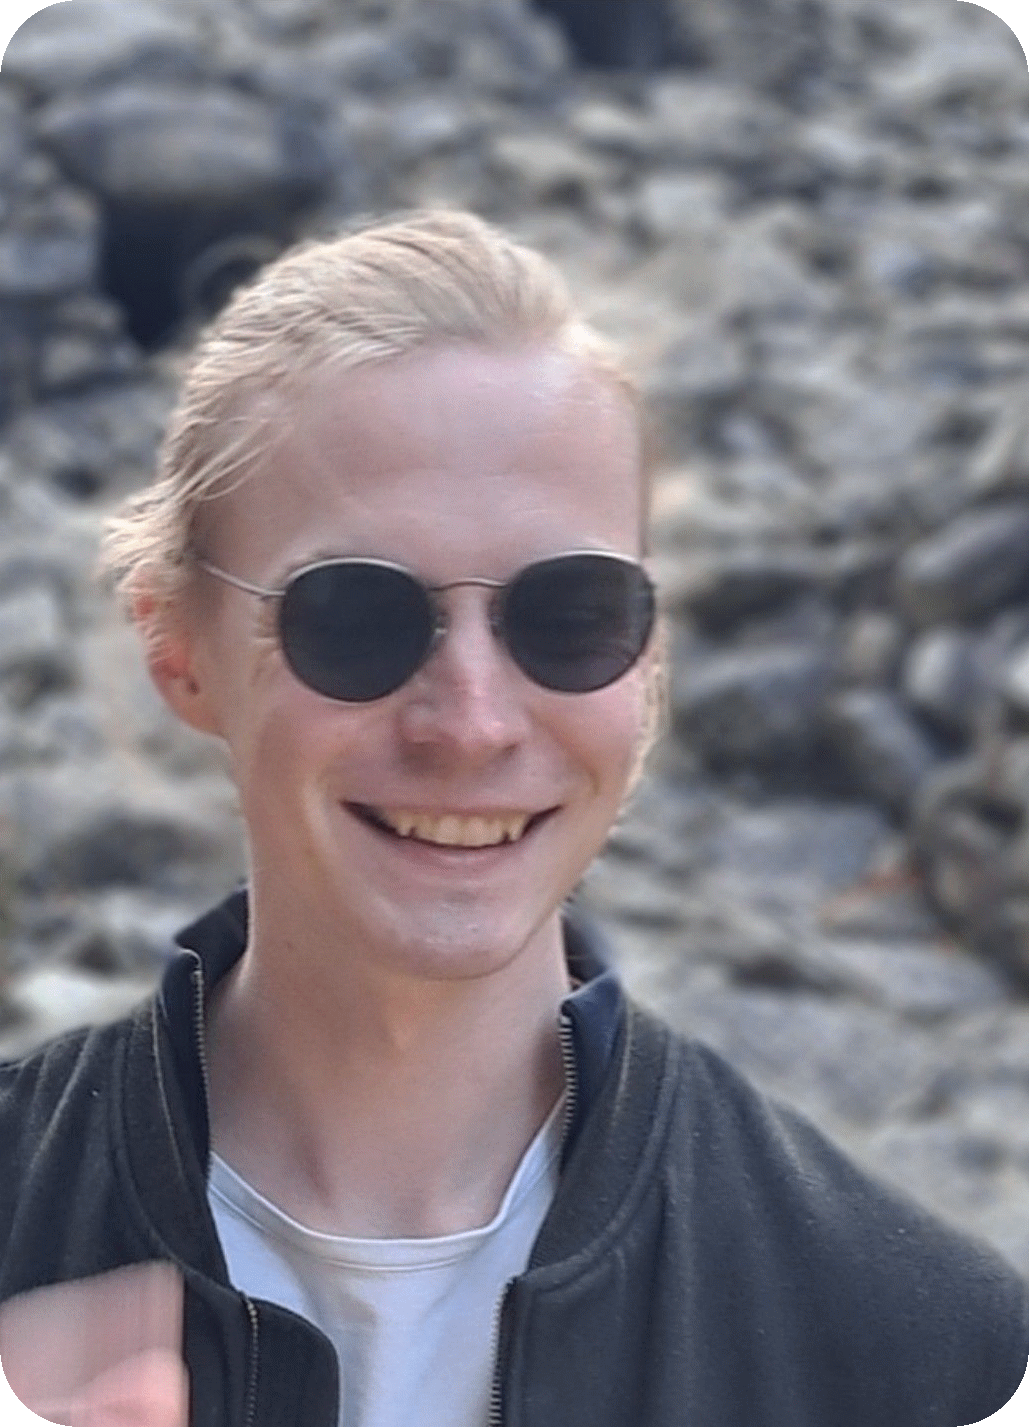
\includegraphics[width=0.85\columnwidth]{trimmedProfile.png} \hfill \\
\vspace{0.4em}
\textbf{\LARGE{Oscar Karlsson}} \\
\color{darkgray!80!black}
MSc Science in Engineering\\

\vspace{.25em}
%\mysection{Contact}
{\upshape
\makebox[.3cm]{\footnotesize\faPhone} ~+46 72-155-73-48 \\
\makebox[.3cm]{\footnotesize\faEnvelope} \makeemail \\
\makebox[.3cm]{\footnotesize\faGithub} \makegit \\
\makebox[.3cm]{\footnotesize\faLinkedin} \makeLinkedin \\
}
\vspace{2.25em}
\mysection{Skills}
 \vspace{-.75em}

\begin{itemize}[leftmargin =\widthof{~$\bullet$~}]
\setlength\itemsep{0.1em}
\item Stochastic Modeling
	\begin{itemize}[leftmargin =\widthof{~$\bullet$~}]\footnotesize\vspace{-0.3em}
	\setlength\itemsep{0.1em}
	\item Time Series
	\item Financial Modeling
	\item Modern Regression Techniques
	\end{itemize}
\item Machine Learning
	\begin{itemize}[leftmargin =\widthof{~$\bullet$~}]\footnotesize\vspace{-0.3em}
	\setlength\itemsep{0.1em}
	\item Reinforcement Learning
	\item Neural Networks and Deep Learning
	\item Optimization for Learning
	\end{itemize}
\item Applied Statistics
	\begin{itemize}[leftmargin =\widthof{~$\bullet$~}]\footnotesize\vspace{-0.3em}
	\setlength\itemsep{0.1em}
	\item Markov Processes
	\item Monte Carlo and MCMC
	\end{itemize}
\item Optimal Control
	\begin{itemize}[leftmargin =\widthof{~$\bullet$~}]\footnotesize\vspace{-0.3em}
	\setlength\itemsep{0.1em}
	\item Stochastic Optimal Control
	\item Learning Based Control
	\end{itemize}
\item Programming and Data Handling
	\begin{itemize}[leftmargin =\widthof{~$\bullet$~}]\footnotesize\vspace{-0.3em}
	\setlength\itemsep{0.1em}
	\item[{\makebox[.15cm]{\faPython}}] Python
	\item[{\makebox[.15cm]{\faRProject}}] R
	\item[{\makebox[.15cm]{\faJava}}] Java
	\item[{\makebox[.15cm]{\faDatabase}}] SQL
	\item[{\makebox[.15cm]{\faFileExcel}}] Excel
	\end{itemize}
\end{itemize}

\vspace{1.25em}
\mysection{Languages}
 \vspace{-.75em}
\begin{itemize}[leftmargin =\widthof{~$\bullet$~}]
\setlength\itemsep{0.1em}
\item English -- Native Fluency
\item Swedish -- Native Fluency
\end{itemize}



%%%%%%%%%%%%%
% Fill the right hand column
%%%%%%%%%%%%%
\switchcolumn
\mysection{Professional Summary}
I am a recently graduated Engineer with a focus on financial modeling, machine learning and control theory. I'm a curious problem solver, always looking to expand my horizons. I thrive when working in a team, truly great accomplishments are made when you build on each other's strengths, benefit from shared knowledge and develop together.

\vspace{1.5em}

\mysection{Work Experience}
\WExperience{Care assistant - Nighttime}{Lunds Kommun}{May 2023 - Aug 2023}{Lund, Skåne Län}
\begin{itemize}[leftmargin =\widthof{$\bullet$~~~~~}]
\item Individually managed  list of visits, provided medicine by delegation, and adapted to additional and emergency visits requested by clients.
\end{itemize}

\WExperience{Tutoring}{Astronomisk Ungdom}{2022}{Lund, Skåne Län}
\begin{itemize} [leftmargin =\widthof{$\bullet$~~~~~}]
\item Tutored high-school students in Math and Physics for Astronomisk Ungdom
\end{itemize}

\vspace{0.3em}
\WExperience{Warehouse employee}{IKEA Indirect Material and Services AB}{July 2021 - Aug 2021 $\vert$ June 2020 - Aug 2020}{Älmhult, Kronobergs Län}
\begin{itemize} [leftmargin =\widthof{$\bullet$~~~~~}]
\item Operated forklift and handled picking to meet KPIs in largely unsupervised setting
\end{itemize}

\vspace{1.5em}
\mysection{Volunteering}
\WExperience{International Mentor}{Lunds University}{Fall 2021 to Early Spring 2022}{Lund, Skåne Län}
\begin{itemize}[leftmargin =\widthof{$\bullet$~~~~~}]
\item Introduced international students to student life in Lund, as well as assisting with logistical, practical and social elements of studying abroad
\end{itemize}

\vspace{0.3em}
\WExperience{Auditor/Cashier}{LARA - Lund Aerospace and Rocketry Association}{2021-2024}{Lund, Skåne Län}
\begin{itemize}[leftmargin =\widthof{$\bullet$~~~~~}]
\item Served as an auditor (2021), and the cashier (2022-2024), as well as led smaller projects
\end{itemize}

\vspace{.75em}
\mysection{Education}
\WExperience{Master of Science in Engineering (Civilingenjör i Teknisk Fysik)}{Aug 2020 - June 2025}{Lund University}{Lund Skåne Län}
\begin{itemize}[leftmargin =\widthof{$\bullet$~~~~~}]
\item Specialized in Machine Learning (AI), Optimal Control and statistical tools for Time Series and Financial applications
\item Wrote Master's thesis with Nordea in Copenhagen \\ \textit{Better hedging of CVA with Reinforcement Learning} \\ Supervisors: Dr. Magnus Wiktorsson, Lund University; Shengyao Zhu, Nordea
\item Strong foundation in math, physics and programming from core coursework
\end{itemize}

\WExperience{IB Bilingual Diploma}{Completed 2019}{Katedralskolan Lund}{Lund Skåne Län}
\begin{itemize}[leftmargin =\widthof{$\bullet$~~~~~}]
\item Native Fluency in English and Swedish having lived in the United States and Sweden as well as completed the IB program
\end{itemize}

\end{paracol}


\newpage
\setstretch{1}
\raggedright
\mysection{Projects}
\PExperience{\MastersTitle}{Spring 2025}{Python, PDEs/SDEs, ML, Stochastic Optimal Control}
\begin{itemize}
\item Wrote My Master's thesis under the supervision of Zhu Shengyao at the Nordea XVA desk and Dr. Magnus Wiktorsson from Lunds University, on applying ML techniques to hedge CVA (Credit Value Adjustment) on Interest Rate Swaps.
	\begin{itemize} 
		\item The project involved constructing a simulated market environment capturing key risks, and complexities associated with both CVA and IRS products. After much consideration, we used a one factor Hull White model for interest rate 		modeling, with a real world calibrated forward curve. We modeled defaults as being driven by a JCIR model, and generated data with various correlations between interest rate and default.
		\item The project further involved designing and training a Reinforcement Learning Network to minimize risk metrics, which is handled as a stochastic optimal control problem. This stage involved network creation, RL environment design, from reward function to transformation of observations and outputs and problem aware hyper-parameter tuning.
		\item The paper is available from Lunds University \href{http://lup.lub.lu.se/student-papers/record/9197473}{ \scriptsize \faLink}, and the code is made available on GitHub\smallgit{https://github.com/Squid-oid/cva_risk_management_thesis}.
	\end{itemize}
\end{itemize}

\PExperience{Minor Programming Projects}{2020-2025}{Python, Numpy, Java, SQL, Data Scraping, Data Structures, Data Engineering}
\begin{itemize}
\item Produced a variety of hobby programming projects through my time at the Uni for fun and to apply knowledge gained, some selected examples are:
	\begin{itemize}\normalsize 
		\item Self taught SQL with mockup of rock-climbing tracking app~(ongoing). Interfaced between locally hosted MySQL server and Python through the use of pyodbc. Proved knowledge in both DDL in setting up database and DML through 				automated and manual insertion of synthetic data and construction of complex queries. \smallgit{https://github.com/Squid-oid/SQL}
		\item Coded a 2d physics engine to simulate objects bouncing in a 2d space as a way to test discretization models in a practical application. Utilized pysdl2 and PIL libraries for graphics creation and handling. \smallgit{https://github.com/Squid-oid/physics-fun}
		\item Built numerous small tools and experiments in Python and other languages. Fields range from comparing ML models' performance on synthetic data to practice tools for music.
	\end{itemize}
\end{itemize}

\vfill
\setstretch{0.9}
\mysection{Courses in Selection}
An electronically stamped and verifiable copy of my full degree is available on request. \\ \vspace{1em}
\WExperience{Financial Statistics}{Grade 5, Pass With Distinction}{2024 Fall}{A Level $\vert$ 7.5hp}\\ \vspace{1em}
\WExperience{Financial Management}{Grade 4, Pass With Credit}{2024 Fall}{A Level $\vert$ 6.0hp}\\ \vspace{1em}
\WExperience{Valuation of Derivative Assets}{Grade 5, Pass With Distinction}{2024 Fall}{A Level $\vert$ 7.5hp}\\ \vspace{1em}
\WExperience{Optimization for Learning}{Grade 4, Pass With Credit}{2024 Fall}{A Level $\vert$ 7.5hp}\\ \vspace{1em}
\WExperience{Network Dynamics}{Grade 5, Pass With Distinction}{2024 Spring}{A Level $\vert$ 7.5hp}\\ \vspace{1em}
\WExperience{Linear and Logistic Regression}{Grade 4, Pass With Credit}{2024 Spring}{A Level $\vert$ 7.5hp}\\ \vspace{1em}
\WExperience{Monte Carlo and Empirical Methods for Stochastic Inference}{Grade 5, Pass With Distinction}{2024 Spring}{A Level $\vert$ 7.5hp}\\ \vspace{1em}
\WExperience{Learning Based Control}{Grade 4, Pass With Credit}{2024 Spring}{A Level $\vert$ 7.5hp}\\ \vspace{1em}
\WExperience{Mathematical Statistics, Time Series Analysis}{Grade 4, Pass With Credit}{2023 Fall}{A Level $\vert$ 7.5hp}\\ \vspace{1em}
\WExperience{Markov Processes}{Grade 5, Pass With Distinction}{2023 Fall}{G2 Level $\vert$ 7.5hp}\\  \vspace{1em}
\vfill
\mysection{Programming Languages, Libraries and Computer Literacy}
\textbf{Languages}: Java,  Python,  R, C (basics),  Matlab, SQL \newline
\textbf{Libraries/Frameworks}: Python: pandas,  numpy, statsmodel, tensorflow,  sklearn, torch, SB3 $\vert$ \quad R: MASS,  dpylr  \newline
\textbf{Technologies}: Github,  Jupyter \& Python Notebooks,  Linux,  Windows and Office including Excel,  TeX, Virtual Environments

\end{document}
